% !TEX root = ../main.tex
\section{Deployment}

The product is a Streamlit \cite{streamlit} web app (\texttt{app.py}), the last stage of the pipeline in
Figure~\ref{fig:pipeline}. The catalog embeddings are computed once during training and saved, so the app
never re-encodes the catalog. On start-up it loads the catalog, embeddings and encoder into memory once
(\texttt{@st.cache\_resource}); each search then needs one encoding of the query and one similarity
calculation against the 16,137 stored vectors. The app reads \texttt{model\_selection.json} and loads
whichever model scored best, so the deployed model always matches the latest evaluation.

\begin{figure}[H]
\centering
\begin{tikzpicture}[node distance=0.3cm, every node/.style={font=\footnotesize, align=center},
                    box/.style={draw=accent, rounded corners=2pt, minimum height=0.9cm, text width=2.5cm},
                    >={Stealth[length=4pt]}]
  \node[box] (api) {Stack Exchange API};
  \node[box, right=of api] (col) {collection\\\texttt{questions.csv}};
  \node[box, right=of col] (pre) {preprocessing\\\texttt{questions\_}\\\texttt{clean.csv}};
  \node[box, right=of pre] (tr) {training\\\texttt{outputs/}};
  \node[box, right=of tr] (app) {app.py\\(Streamlit)};
  \foreach \a/\b in {api/col, col/pre, pre/tr, tr/app} \draw[->] (\a) -- (\b);
  \draw[->] (pre.south) |- ++(0,-0.4) -| (app.south);
\end{tikzpicture}
\caption{End-to-end pipeline. \texttt{config.json} holds the settings shared by every stage.}
\label{fig:pipeline}
\end{figure}

The app runs locally. The submitted folder contains everything it needs: the app code, requirements,
configuration, the 50\,MB cleaned catalog and the three files produced by training. It starts with the commands in Listing~\ref{lst:run}.
\notebooklisting[bash]{snippets/run_app.sh}{Installing dependencies and starting the app locally.}{lst:run}
The first launch downloads the MiniLM weights (about 90\,MB); after that everything runs on a CPU.

The deployed product is available at
\url{https://question-recommendation.streamlit.app/}, running the same
\texttt{app.py} with the catalog and model files included in the submission.

In use (Figure~\ref{fig:app}), the ten closest answered questions appear ranked by match percentage,
each with a link, tags, an accepted-answer marker and a preview.

\begin{figure}[H]
  \centering
  \fbox{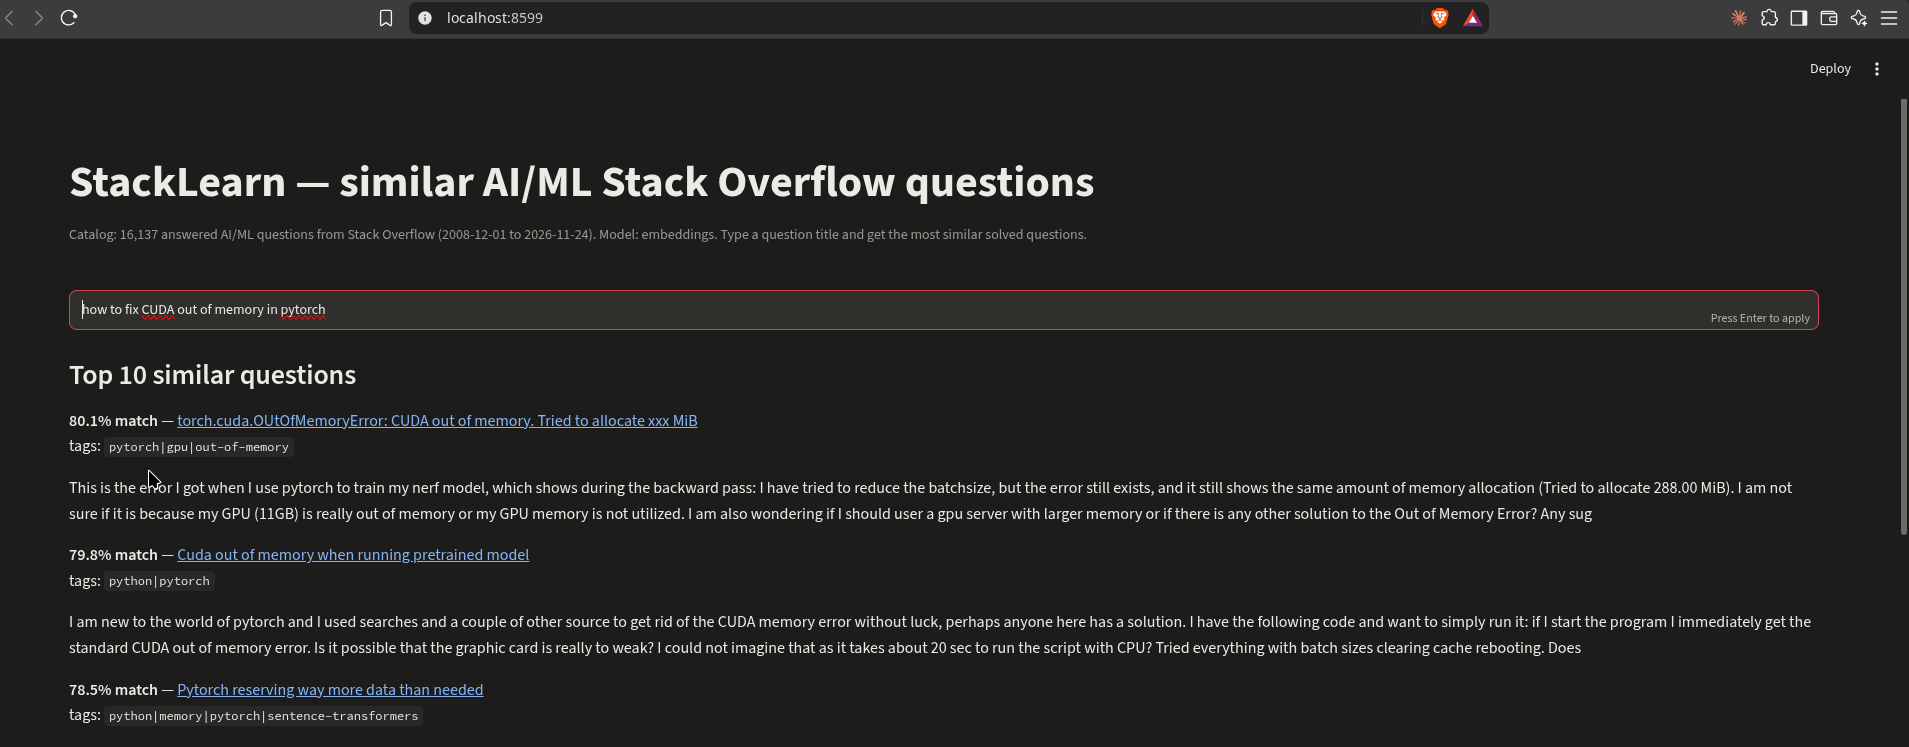
\includegraphics[width=0.97\linewidth]{figures/app.png}}
  \caption{StackLearn answering ``how to fix CUDA out of memory in pytorch''. The top three results
  are all CUDA out-of-memory questions (80.1\%, 79.8\% and 78.5\% match).}
  \label{fig:app}
\end{figure}
